\chapter{An example module}
To bring together everything specified in the API chapter, an example will do nicely. In essence, this is a very basic
module that collects global CPU usage (based on the original cpuTime module). Replace cpuTime with the name of the
module that you yourself are creating, of course.

\section{The project directory}
First off, a project directory is required. A template is provided; simply create a copy of it.

\small{\texttt{
\$ cp -r module/templateModule module/modules/cpuTime
}}

Modify the configuration files as required (change the name of the module, for example); perhaps add a default
configuration item, as shown in Figure \ref{exampleModuleConfig}. 

\begin{figure}[h]
  \small{\texttt{%
module cpuTime \\
\\
set collector=collector.so \\
set polisher=polisher.so \\
\\
set interval=50000
  }}
  \caption{Example module configuration file.\label{exampleModuleConfig}}
\end{figure}

\section{The collector}

The next step is to implement the collector portion of the module. Remove the file entitled ``dummy.c'' from the
collector/ subdirectory of the module root, and instead create a file called ``collector.c''. Or, ``cputime.c'', if you
want. Whatever you like, goes.

Listing \ref{exampleCollector} shows collector.c for the example cpuTime module.

\lstset{%
  language=C,		% This is a C listing . . .
  basicstyle=\tiny,	% Make the text smaller.
  numbers=left,		% Put the line numbers on the left . . .
  numberstyle=\tiny,  	% Make the numbers tiny . . .
  showspaces=false,	% Don't show spaces.
  showtabs=false,	% Nor tabs.
  showstringspaces=false,
  frame=shadowbox,	% Put the listing inside a shadowbox.
  columns=fixed,	% Ensure that the text is nicely fixed into columns.
  caption={Example collector, collector.c},
  label={exampleCollector}
}
\begin{lstlisting}
#include <time.h>
#include <signal.h>
#include <stdlib.h>
#include <sys/time.h>
#include <sys/times.h>
#include <sys/resource.h>
#include <sys/timerfd.h>
#include <pthread.h>
#include <unistd.h>

#include "collector/Interface.h"

AC_moduleDefinition();

int ACM_timerFd;
pthread_t ACM_threadID;
int ACM_running;

static void *ACM_sendTime(void *unused) {
    ACM_running = 1;
    while(ACM_running) {
	uint64_t exp;
	read(ACM_timerFd, &exp, sizeof(exp));
	if(!AC_hasCollectionBegun()) continue;
	
	AC_DataPacket packet;
	struct rusage ru;
	getrusage(RUSAGE_SELF, &ru);
	
	uint64_t value = (ru.ru_utime.tv_sec * 1000000000)
	    + (ru.ru_utime.tv_usec * 1000);
	
	packet.dataSource.timestamp = AC_timestamp();
	packet.dataSource.moduleID = AC_moduleID();
	packet.data = &value;
	packet.dataSize = sizeof(value);
	AC_writePacket(&packet);
    }
    return NULL;
}

void __attribute__((constructor)) AC_constructor() {
    /* NOTE: TFD_CLOEXEC was introduced in Linux 2.6.27; timerfd_create() is
	Linux-specific. */
    if((ACM_timerFd = timerfd_create(CLOCK_REALTIME, TFD_CLOEXEC)) == -1) {
	printf("Failed to create timer . . .\n");
	return;
    }
    
    struct itimerspec its;
    
    int interval = AC_configurationInt("cpuTime", "interval");
    if(interval == 0) {
	/* The default interval is 10 times per second, or every 100 ms. */
	interval = 100000;
    }
    interval *= 1000;
    
    its.it_interval.tv_sec = interval / 1000000000;
    its.it_interval.tv_nsec = interval % 1000000000;
    
    its.it_value.tv_sec = interval / 1000000000;
    its.it_value.tv_nsec = interval % 1000000000;
    
    timerfd_settime(ACM_timerFd, 0, &its, NULL);
    
    pthread_create(&ACM_threadID, NULL, ACM_sendTime, NULL);
    
    AC_registerModule("cpuTime");
}

void __attribute__((destructor)) AC_destructor() {
    ACM_running = 0;
    pthread_join(ACM_threadID, NULL);
}

\end{lstlisting}

The code should be relatively self-explanitory. Reading the man pages for several of the used system calls may be a
good idea, however. One important point to make: the value of the eight-byte data inside the generated DataPackets is a
64-bit, unsigned integer representing the CPU time used by the program.

\section{The polisher}

For this example module, the polisher code is short and sweet, so to speak. No polishing must be done to the data; it
is in a perfectly acceptable state as it stands. However, not creating a polisher module is currently not an
option.\footnote{Patches welcome!}

Thus, without any further ado.

\lstset{
  caption={Example polisher, Polisher.h header.},
  label={examplePolisherHeader}
}
\begin{lstlisting}
#ifndef Polisher_H
#define Polisher_H

#include "polisher/Polisher.h"

class CpuTimePolisher : public PolisherInterface {
public:
    CpuTimePolisher();
    virtual ~CpuTimePolisher();
private:
public:
    virtual DataPacket *handlePacket(DataPacket *packet);
};

#endif
\end{lstlisting}

\lstset{
  caption={Example polisher, Polisher.cpp source file.},
  label={examplePolisherSource}
}
\begin{lstlisting}
#include "Polisher.h"

CreateInstantiationFunction(CpuTimePolisher)

CpuTimePolisher::CpuTimePolisher() {

}

CpuTimePolisher::~CpuTimePolisher() {

}

DataPacket *CpuTimePolisher::handlePacket(DataPacket *packet) {
	return packet;
}
\end{lstlisting}

The \emph{handlePacket()} method is very simplistic. All it does is return the packet it is given \ldots but, then
again, that is all that is required of it.

And again, the code should be self-explanitory.

\section{The renderer}
The renderer module is far more complex than even the other two modules placed together. Two classes must be
subclassed, as previously mentioned, and a third must be instantiated. To start off with the basics . . .

\lstset{
  caption={Example renderer, Controller.cpp source file.},
  label={exampleRendererController}
}
\begin{lstlisting}
#include "renderer/Controller.h"
#include "DataCache.h"
#include "GlobalUsageRenderer.h"

extern "C" {

RendererController *Instantiate() {
    RendererController *controller = new RendererController();
    ConcreteRendererFactory *factory = new ConcreteRendererFactory();
    CpuTimeDataCache *dataCache = new CpuTimeDataCache();
    controller->setDataCache(dataCache);
    controller->setFactory(factory);

    factory->registerRenderer("Global CPU usage",
	new GlobalUsageRenderer(dataCache));

    return controller;
}

} // extern "C"
\end{lstlisting}

Now, after this, two more classes are (obviously) required; \emph{CpuTimeDataCache} and \emph{GlobalUsageRenderer}. The
definitions for the two:

\lstset{
  caption={Example renderer, DataCache.h header file.},
  label={exampleRendererDataCacheHeader}
}
\begin{lstlisting}
#ifndef DataCache_H
#define DataCache_H

#include <vector>

#include "renderer/AbstractDataCache.h"
#include "renderer/DataCoord.h"

class CpuTimeDataCache : public AbstractRendererDataCache {
public:
    virtual ~CpuTimeDataCache() {}
    
    typedef std::vector<DataCoord> DataVector;
private:
    DataVector m_dataVector;
    uint64_t m_lastCpuTime;
public:
    const DataVector &dataVector() const { return m_dataVector; }
    virtual void processPacket(DataPacket *packet);
};

#endif

\end{lstlisting}

\lstset{
  caption={Example renderer, GlobalUsageRenderer.h header file.},
  label={exampleRendererGURendererHeader}
}
\begin{lstlisting}
#ifndef GlobalUsageRenderer_H
#define GlobalUsageRenderer_H

#include "renderer/AbstractRenderer.h"
#include "DataCache.h"

class GlobalUsageRenderer : public AbstractRenderer<CpuTimeDataCache> {
public:
    GlobalUsageRenderer(CpuTimeDataCache *dataCache);
    virtual ~GlobalUsageRenderer() {}
private:
public:
    virtual void renderRange(VisualizationWrapper *visualization,
	const DataRange &range, bool *abort);
    virtual DataRange defaultRange() const;
};

#endif
\end{lstlisting}

Again, these two source files are very simple; they both define implementations of classes that have pure virtual
methods.

The definitions for the previous two headers:

\lstset{
  caption={Example renderer, DataCache.cpp source file.},
  label={exampleRendererDataCacheSource}
}
\begin{lstlisting}
#include "DataCache.h"

void CpuTimeDataCache::processPacket(DataPacket *packet) {
    uint64_t cpuTime = *(uint64_t *)packet->data;
    if(m_dataVector.size() == 0) {
    m_dataVector.push_back(DataCoord(packet->dataSource.timestamp, 0.0));
    }
    else {
	uint64_t ddiff = cpuTime - m_lastCpuTime;
	Timestamp tdiff = packet->dataSource.timestamp - m_dataVector.back().time();
	
	double usage = ddiff / (double)tdiff;
	
	m_dataVector.push_back(DataCoord(packet->dataSource.timestamp, usage));
    }
    m_lastCpuTime = cpuTime;
}
\end{lstlisting}

\lstset{
  caption={Example renderer, GlobalUsageRenderer.cpp source file.},
  label={exampleRendererGURendererSource}
}
\begin{lstlisting}
#include <algorithm>

#include "GlobalUsageRenderer.h"

GlobalUsageRenderer::GlobalUsageRenderer(CpuTimeDataCache *dataCache)
    : AbstractRenderer<CpuTimeDataCache>(dataCache) {
    
}

static bool compareCoords(const DataCoord &one, const DataCoord &two) {
    if(one.time() < two.time()) return true;
    return false;
}

void GlobalUsageRenderer::renderRange(VisualizationWrapper *visualization,
	const DataRange &range, bool *abort) {
    const CpuTimeDataCache::DataVector &dataVector = dataCache()->dataVector();
    
    DataCoord c;
    
    c.setTime(range.beginTime());
    c.setData(0.0);
    
    CpuTimeDataCache::DataVector::const_iterator begin =
	std::lower_bound(dataVector.begin(), dataVector.end(), c, compareCoords);
	
    if(begin == dataVector.end()) {
	/* Then the visualization is out of range. */
	return;
    }
    else if(begin != dataVector.begin()) --begin;
    
    c.setTime(range.endTime());
    
    CpuTimeDataCache::DataVector::const_iterator end =
	std::upper_bound(dataVector.begin(), dataVector.end(), c, compareCoords);
    
    if(end == dataVector.begin()) {
	/* Then the visualization is out of range. */
	return;
    }
    else if(end != dataVector.end()) ++end;
    
    visualization->lock();

    for(; begin != (end-1); ++begin) {
	visualization->drawLine((*begin), *(begin + 1));
    }
    
    visualization->unlock();
}

DataRange GlobalUsageRenderer::defaultRange() const {
    const CpuTimeDataCache::DataVector &dataVector = dataCache()->dataVector();
    return DataRange(DataCoord(dataVector.front().time(), 0.0),
	DataCoord(dataVector.back().time(), 1.5));
}

\end{lstlisting}

To fully understand the code in the DataCache type, a quick background in calculating CPU usage is required. In
UNIX-based operating systems, the kernel keeps track of the culumative processing time a process has consumed. This
makes it easy to calculate the CPU usage for a given period, given $\Delta t$ and $\Delta C_{time}$:

\begin{center}
  \begin{math}
    usage_{percent} = \Delta C_{time} / \Delta t
  \end{math}
\end{center}

Note that this calculates a value between 0 and $n_{cores}$, where $n_{cores}$ is the number of SMP cores the computer
in question posseses.\footnote{This is actually, for reference, similar to how load averages are calculated.}

\section{Compiling}
The next step is to add the module to the Aesalon build system. Contained within the \emph{module/modules/} directory
is a file called \emph{build\_list}. Add the name of the directory to the end of the \emph{set()} call. Run \emph{make},
and your module should be built automatically.

\section{Output}
Of course, this sort of visualization is very, very basic, and doesn't look like very much.
Figure \ref{exampleModuleOutput} shows the basic output produced by this module.

\begin{figure}[t]
  \begin{center}
    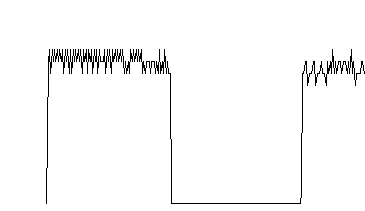
\includegraphics[scale=0.25]{exampleModuleScreenshot}
  \end{center}
  \caption{A screenshot of the example cpuTime module. \label{exampleModuleOutput}}
\end{figure}
